\section{EC 3.14}
\textbf{Exercise 14.0.1} (Market model definition). \textit{Provide the definition of the market model used by Arrow and Debreu.}\\

Consider a market model as follows:
\begin{itemize}
\item $N=\{1, \ldots, n\}$ is the set of players;
\item $K=\{1, \ldots, k\}$ is the set of perfectly divisible commodities;
\item $x_{i} \in \mathbb{R}_{+}^{k}$ with $i \in N$ is a vector of $k$ elements, where $x_{i, j},$ denoting the element in the $j$-th position of the vector, represents the amount of commodity $j$ available to player $i$;
\item $e_{i} \in \mathbb{R}_{+}^{k}$ with $i \in N$ is the initial endowment of player $i$ and $e_{i, j}$ is the initial endowment for commodity $j$;
\item $u_{i}: \mathbb{R}_{+}^{k} \rightarrow \mathbb{R}_{+}$ is the utility function of player $i$ that is continuous and concave;
\item $p \in \mathbb{R}_{+}^{k}$ is a vector of $k$ elements, where $p_{j},$ denoting the element in the $j$-th position of the vector, represents the price of commodity $j$.
\end{itemize}
Each player maximizes her utility function under budget constraints by buying/selling commodities. Formally, we have:
\[
\begin{array}{cl}
\max _{x_{i}} & u_{i}\left(x_{i}\right) \\
\text { s.t. } & p \cdot x_{i} \leqslant p \cdot e_{i}
\end{array}
\]
where $p \cdot e_{i}$ represents the budget available to player $i,$ while the argument of the above optimization problem, denoted by $x_{i}^{*},$ is the best amount of commodity for player $i$ given the market prices and the budget constraints. Notice that the above optimization problem does not take into account any constraint related to the amount of commodities available in the market. Thus, in principle, the above optimization problem may return a $x_{i}^{*}$ that is not implementable in practice, requiring an excessive amount of commodities larger than that one actually available in the market.\\

\textbf{Exercise 14.0.2} (Market clearing). \textit{Provide the definition of market clearing.}\\

The market clears when the total amount of commodities $x=\sum_{i \in N} x_{i}$ equals to total amount of initial endowments $e=\sum_{i \in N} e_{i}$.\\
Notice that, when the price vector is arbitrary, there is no guarantee that the market clears. For instance, as already mentioned above, it may happen that the vector $x$ is larger than $e$ for some commodities. The market clearing property is of paramount importance and depends on the price vector. Indeed, when this property holds, each player in the market acts independently from the others. In other words, each player negotiates with a fictitious player corresponding to the market. This allows one to neglect the direct interaction between the players when searching for the market outcome.

Thus, the study of the conditions under which the market clears is crucial. This is stated by the Arrow-Debreu theorem.\\

\textbf{Exercise 14.0.3} (Arrow-Debreu equilibrium). \textit{Provide the definition of the Arrow-Debreu equilibrium and argue the meaning of the result.}\\

There is always a price vector $p^{*}$ such that $\sum_{i \in N} x_{i}^{*} \leqslant e$ and $p^{*}$ is Pareto efficient for the players.\\
The problem of finding an Arrow-Debreu equilibrium is slightly different from the problem of finding a Nash equilibrium. On the one hand, each player behaves rationally, maximizing her utility function, as in a Nash equilibrium. In particular, the problem reduces to the problem of finding a Nash equilibrium when prices are fixed. On the other hand, prices are part of the problem. Thus the problem of finding an Arrow-Debreu equilibrium can be formulated as the problem of finding prices satisfying some conditions under the equilibrium constraints of the players. Interestingly, the problem of finding an Arrow-Debreu equilibrium presents the same computational properties of the problem of finding the Nash equilibrium, as stated below.\\
(Arrow-Debreu equilibrium complexity). The problem of finding a Arrow-Debreu market equilibrium is \textsf{PPAD}-complete even when all traders use additively separate, piecewise-linear and concave utility functions.

\section{EC 3.15}
\textbf{Exercise 15.0.1} (Leader-Follower equilibrium definition). \textit{Provide the definition of the Leader-Follower equilibrium with 2 players.}\\

The problem of finding a Leader–Follower equilibrium is formulated as:
\begin{figure}[H]
\centering
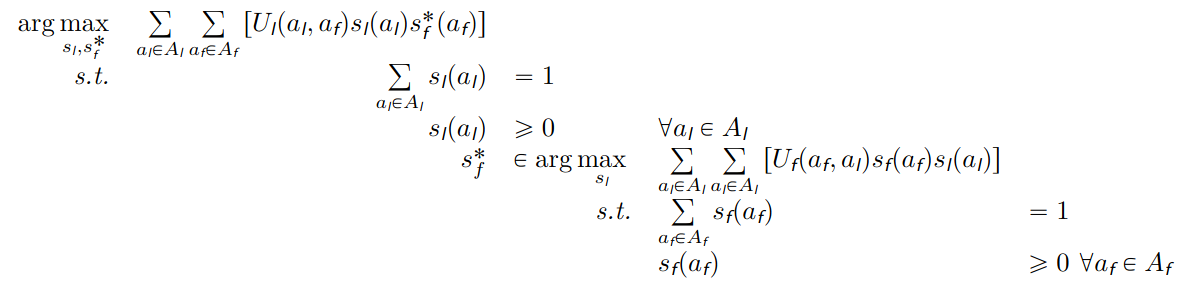
\includegraphics[width=\textwidth]{images/img_3_15_01.png}
\end{figure}

\textbf{Exercise 15.0.2} (Leader-Follower equilibrium properties). \textit{Describe the properties of the Leader-Follower equilibrium with 2 players.}\\

A Stackelberg equilibrium always exist when ties are broken in favour of the leader.\\
A Stackelberg equilibrium may not exist when ties are not broken in favour of the leader.\\
With 2 players (one leader and one follower), committing to a strategy never hurts the leader when ties are broken in its favour.\\
Equivalently, under those conditions, the best Nash for the leader is never strictly better than the Stackelberg equilibrium for the leader.\\

\textbf{Exercise 15.0.3} (Leader-Follower equilibrium example). \textit{Given a 2-player normal-form game with 2 actions per player, find a Leader-Follower equilibrium.}\\

Consider the following 2-player game with 2 actions per player:
\begin{figure}[H]
\centering
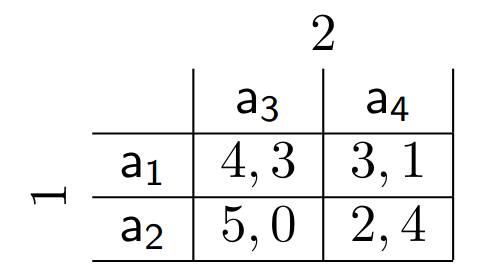
\includegraphics[width=0.3\textwidth]{images/img_3_15_02.png}
\end{figure}
Under the constraint that the follower plays $\mathsf{a_3}$, the best strategy of the leader and the corresponding value is:
\[
s_{l}=\begin{cases}
\frac{2}{3} & \mathsf{a_1} \\
\frac{1}{3} & \mathsf{a_2}
\end{cases} \quad \quad v_{l}=\frac{13}{3}
\]
while under the constraint that the follower plays $\mathsf{a_4}$, the best strategy of the leader and the corresponding value is:
\[
s_{l}=\begin{cases}
\frac{2}{3} & \mathsf{a_1} \\
\frac{1}{3} & \mathsf{a_2}
\end{cases} \quad \quad v_{l}=\frac{8}{3}
\]
Under the assumption that the follower breaks ties in favor of the leader, the equilibrium is:
\[
s_{l}=
\begin{cases}
\frac{2}{3} & \mathsf{a_1} \\
\frac{1}{3} & \mathsf{a_2}
\end{cases} \quad \quad
s_{f}=
\begin{cases}
1 & \mathsf{a_1} \\
0 & \mathsf{a_2}
\end{cases}
\]
We show that no equilibrium exists if the follower breaks ties in a different way. For any fully mixed $s_f$ played when $s_l = (\frac{2}{3}, \frac{1}{3})$, the utility function of the leader has a superior at $s_l = (\frac{2}{3}, \frac{1}{3})$ but the maximum does not exist. Indeed, the best strategy of the leader is $s_l = (\frac{2}{3} + \epsilon, \frac{1}{3}) + \epsilon$ with $\epsilon \rightarrow 0$, but $\epsilon$ cannot be $0$. In other words, the limit does not exist. The expected utility of the leader is depicted in the figure below.
\begin{figure}[H]
\centering
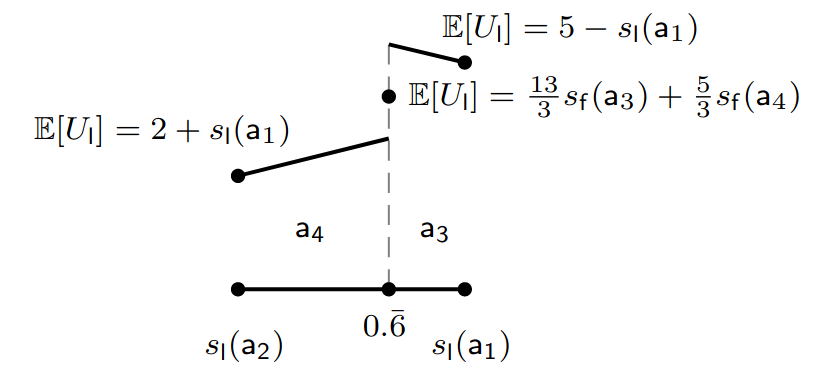
\includegraphics[width=0.5\textwidth]{images/img_3_15_03.png}
\end{figure}

\textbf{Exercise 15.0.4} (Leader-Follower equilibrium formulation). \textit{Provide the mathematical programming formulation to find a Leader-Follower equilibrium with 2 players.}\\

The Leader–Follower equilibrium can be found by solving the following mathematical programming problem:
\begin{figure}[H]
\centering
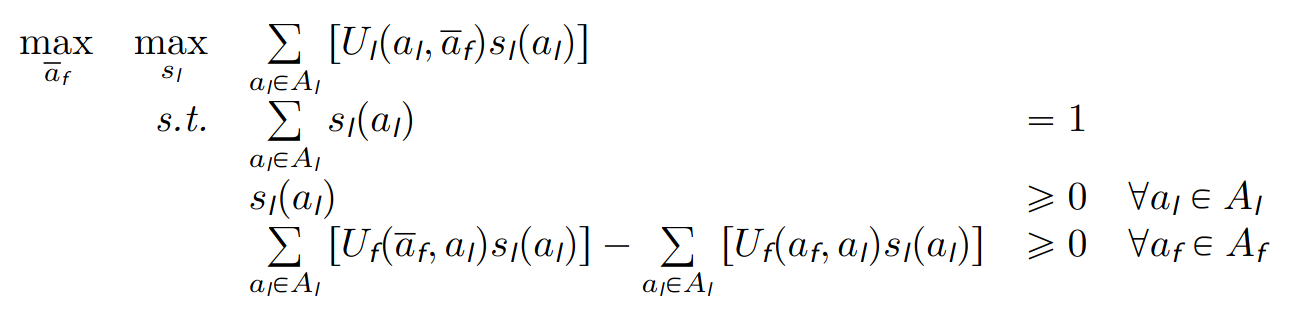
\includegraphics[width=0.8\textwidth]{images/img_3_15_04.png}
\end{figure}
whose nature is Multi–Linear Program (Multi–LP).\\

\textbf{Exercise 15.0.5} (Finding a Leader-Follower equilibrium). \textit{Given a 2-player normal-form game, find a Leader-Follower equilibrium by means of AMPL + GUROBI.}\\
\begin{verbatim}
-----------------------------file.mod-----------------------------

set A;

param Ul{A, A};
param Uf{A, A};
param AF;

var sl{A} >= 0;

maximize objective: sum{a in A} Ul[al, AF] * sl[al];

subject to constraint1{af in A}: sum{al in A} Uf[al, AF] * sl[al] 
                    - sum{al in A} Uf[al, af] * sl[al]>= 0;
subject to constraint2: sum{al in A}: sl[al] = 1;

-----------------------------file.dat-----------------------------

set A := 1 2 3 4;

param Ul: 1 2 3 4 :=
	1   1 0.5 0.5 0.5
	2 0.5   1 0.5 0.5
	3   1 0.5   1 0.5
	4 0.5 0.5 0.5   1;

param Uf: 1 2 3 4 :=
	1   1 0.4 0.3 0.3
	2 0.6   0 0.4 0.3
	3 0.7 0.5   0 0.4
	4 0.7 0.7 0.6   0;
	
-----------------------------file.run-----------------------------

model file.mod;
data file.dat;

option solver gurobi;

let AF := 1;
solve;
display AF, objective;

let AF := 2;
solve;
display AF, objective;

let AF := 3;
solve;
display AF, objective;

let AF := 4;
solve;
display AF, objective;

------------------------------------------------------------------
\end{verbatim}

\textbf{Exercise 15.0.6} (Leader-Follower equilibrium complexity). \textit{What is the computational complexity of finding a Leader-Follower equilibrium?}\\

The problem of finding a Leader–Follower equilibrium is in \textsf{FP} class.\\

\textbf{Exercise 15.0.7} (Leader-Follower equilibrium vs.  Nash equilibrium). \textit{Describe the relationships between Leader-Follower equilibrium and Nash equilibrium.}\\

The value of the leader in a Leader-Follower equilibrium is never strictly smaller than the value of the leader in the Nash equilibrium that is best one for the leader.\\
\textit{Proof}. In the worst case for the leader, in the Leader-Follower equilibrium the leader plays her strategy of the Nash equilibrium that is the best for her, while the follower plays in pure strategies. Since the follower breaks ties in favor of the leader, the value of the leader is always (except for degenerate cases) larger than the value she would receive in the Nash.\\
(Leader-Follower vs. Nash strategy). One could question whether in a Leader-Follower equilibrium the leader always plays the strategy she would play in a Nash equilibrium and the follower plays in pure strategy the best response that is the best for the leader. If this property were true, we could find a Nash equilibrium in polynomial time by, at first, finding the Leader-Follower equilibrium (in polynomial time), and then, given the leader's strategy, by finding the strategy that the follower would play in the Nash equilibrium (it can be easily showed that also this step can be done in polynomial time). This would show that $\mathsf{P=PPAD}$. Instead, it can be showed that in a Leader-Follower equilibrium the leader could play actions that she would never play in any Nash equilibrium as remarked below.\\ (Leader-Follower vs. Nash strategy). In a Leader-Follower equilibrium the leader could play actions that she would never play in any Nash equilibrium and the value of the leader in a Leader-Follower equilibrium may be arbitrarily larger than the value in the best for her Nash equilibrium.\\

\textbf{Exercise 15.0.8} (Leader-Follower equilibrium formulation with multi-type follower). \textit{Provide the mathematical programming formulation to find a Leader-Follower equilibrium with 2 players when the follower can be of multiple types.}\\

The Leader-Follower equilibrium,when the follower can be of different types, can be found by solving the following mathematical programming problem (where $k = |\Theta_f|$):
\begin{figure}[H]
\centering
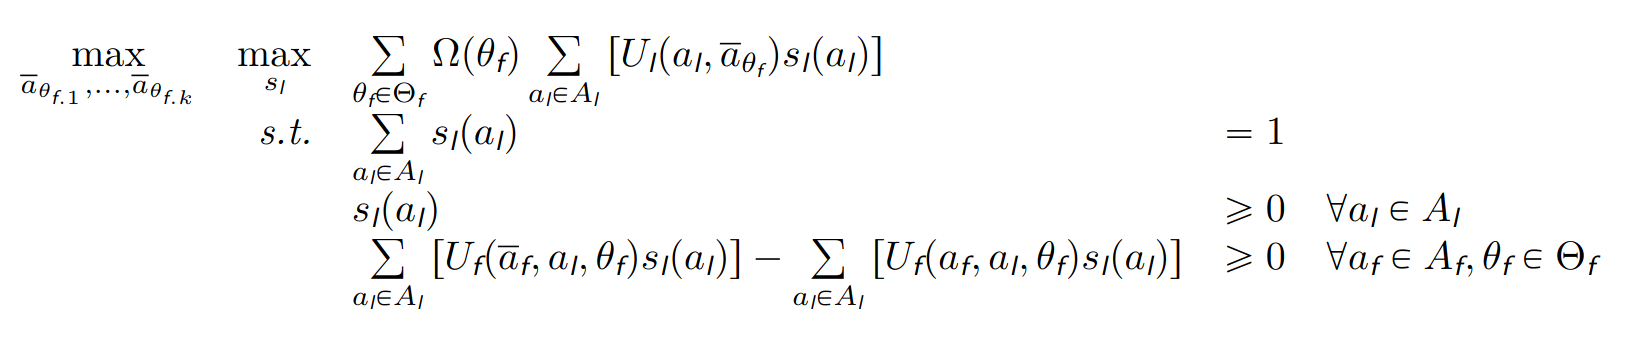
\includegraphics[width=\textwidth]{images/img_3_15_05.png}
\end{figure}
whose nature is Multi–Linear Program (Multi–LP).\\

\textbf{Exercise 15.0.9} (Finding a Leader-Follower equilibrium). \textit{Given a 2-player normal-form game in which the follower can be of multiple types, find a Leader-Follower equilibrium by means of AMPL + GUROBI.}\\
\begin{verbatim}
-----------------------------file.mod-----------------------------

set A;
set T;

param Ul{A, A};
param Uf{A, A, T};
param P{T};
param AF{T};

var sl{A} >= 0;

maximize objective: sum{t in T, a in A} P[t] * Ul[al, AF[t], t] * sl[al];

subject to constraint1{af in A, t in T}: sum{al in A} Uf[al, AF[t], t] * sl[al] 
                    - sum{al in A} Uf[al, af, t] * sl[al]>= 0;
subject to constraint2: sum{al in A} sl[al] = 1;

-----------------------------file.dat-----------------------------

set A := 1 2 3 4;
set T := type1 type2;

param P :=
    type1 0.5
    type2 0.5;

param Ul: 1 2 3 4 :=
	1   1 0.5 0.5 0.5
	2 0.5   1 0.5 0.5
	3   1 0.5   1 0.5
	4 0.5 0.5 0.5   1;

param Uf:
    [*, *, type1]: 1 2 3 4 :=
	    1   0 0.4 0.3 0.3
	    2 0.6   0 0.4 0.3
	    3 0.7 0.6   0 0.4
	    4 0.7 0.7 0.6   0;
    [*, *, type2]: 1 2 3 4 :=
	    1   0 0.7 0.6 0.6
	    2 0.4   0 0.7 0.6
	    3 0.3 0.3   0 0.7
	    4 0.3 0.7 0.4   0;
	
-----------------------------file.run-----------------------------

model file.mod;
data file.dat;

option solver gurobi;

let AF['type1'] := 1;
let AF['type2'] := 1;
solve;
display AF, objective, sl;

let AF['type1'] := 1;
let AF['type2'] := 2;
solve;
display AF, objective, sl;

let AF['type1'] := 1;
let AF['type2'] := 3;
solve;
display AF, objective, sl;

let AF['type1'] := 1;
let AF['type2'] := 4;
solve;
display AF, objective, sl;

...

------------------------------------------------------------------
\end{verbatim}

\textbf{Exercise 15.0.10} (Leader-Follower equilibrium complexity). \textit{What is the computational complexity of finding a Leader-Follower equilibrium when the follower can be of multiple types?}\\


(Multi-LP complexity).The Multi-LP has exponential complexity, enumerating an exponential number of LPs $O(m^k)$, each with a linear number of constraints $O(m \cdot k)$.\\
(Bayesian Leader-Follower complexity with single-type leader). n nThe problem of finding a Leader-Follower equilibrium when the follower can be of different types is in \textsf{FNP}-hard.


\section{EC 3.16}

\textbf{Exercise 16.0.1} (Congestion game definition). \textit{Provide the definition of Congestion game.}\\

A congestion game is a tuple $(N,M, (A_i)_{i \in N}, (c_j)_{j \in M}$ where:
\begin{itemize}
\item $N= \{1,2,\ldots,n\}$ is the set of players;
\item $M= \{1,2,\ldots,m\}$ is the set of resources;
\item $A_i \subseteq \wp (M)$ is the set of action of player $i$, where each action $a$ is a subset of the set of resources;
\item $c_j: N \rightarrow \mathbb{R}$ is a function returning the cost related to resource $j$ when it is used by a given number of players.
\end{itemize}

\textbf{Exercise 16.0.2} (Pure-strategy Nash equilibrium in congestion games). \textit{Prove that every finite congestion game admits at least a pure-strategy Nash equilibrium.}\\
(Pure-strategy Nash equilibrium existence). Every finite congestion game has a pure-strategy Nash equilibrium.\\
\textit{Proof}. Let $\Phi : A \rightarrow \mathbb{R}$ be a function, called potential function, defined as:
$$\Phi(\mathbf{a}) = \sum_{j=1}^{m} \sum_{k=1}^{\textsf{cong}_j (\mathbf{a})} c_j (k)$$
Initially, we show that if, given an action profile $\mathbf{a}$, a player, say $i$, changes its strategy, say from $a_i$ to $a'_i$, we have $\Delta \Phi = \Delta C_i$, where:
$$\Delta \Phi =\Phi\left(a_{i}^{\prime}, \mathbf{a}_{-i}\right)-\Phi(\mathbf{a})$$
$$\Delta C_{i} =C_{i}\left(a_{i}^{\prime}, \mathbf{a}_{-i}\right)-C_{i}(\mathbf{a})$$
That is, we can show that the difference in terms of costs incurred to player $i$ from switching from $a_i$ to $a'_i$ equals the difference of the potential function. The calculations are:
$$C_{i}\left(a_{i}^{\prime}, \mathbf{a}_{-i}\right) -C_{i}(\mathbf{a})=\sum_{j \in a_{i}^{\prime} \backslash a_{i}} c_{j}\left(\operatorname{cong}_{j}(\mathbf{a})+1\right) - \sum_{j \in a_{i} \backslash a_{i}^{\prime}} c_{j}\left(\operatorname{cong}_{j}(\mathbf{a})\right)=\Phi_{i}\left(a_{i}^{\prime}, \mathbf{a}_{-i}\right)-\Phi_{i}(\mathbf{a})$$
Now we show that there is always at least a pure-strategy Nash equilibrium. Consider an algorithm in which at each step a single player changes her strategy by playing her best response (unless the current strategy is already a best response). At each step, the player that makes the move that reduces her cost by $\Delta C_i$ and consequently reduces the potential function. Since $\Phi$ can assume only finite values, the application of such an algorithm eventually returns a local minimum corresponding to an action profile in which no player can reduce further her cost by unilateral deviations. That is, a local minimum of $\Phi$ corresponds to a pure-strategy Nash equilibrium.\\

\textbf{Exercise 16.0.3} (Best-response paths). \textit{Provide the definition of best-response paths and prove that in every finite congestion game all the best-response paths are finite.}\\

A best-response path is a sequence of action profiles such that every pair of consecutive action profiles $a$, $a'$ differ for the action of a single player that, in $a'$, plays her best response.\\

The proof follows a simple algorithm in which, given an action profile,
\begin{enumerate}
\item take a player that is not playing her best response
\item make her to play the best response
\item this leads to a switch in which the cost reduces by a finite value
\item repeat it, until a pure Nash is not reached
\item since at every switch the potential function reduces by a non-infinitesimal value and the potential function is lower bounded, the algorithm must terminate in finite time
\end{enumerate}

\textbf{Exercise 16.0.4} (Finding best-response paths). \textit{Given a congestion game, find a best-response path.}\\

\textcolor{red}{TODO}\\

\textbf{Exercise 16.0.5} (Potential functions). \textit{Provide the definitions of potential functions and discuss the relationships between potential games and congestion games.}\\

(Exact potential function). A function $\Phi: A \rightarrow \mathbb{R}$ is an exact potential function for a game if, for every $a\in A$ and for every $i \in N$, $\Delta \Phi = \Delta C_i$.\\
(Weighted potential function). A function $\Phi: A \rightarrow \mathbb{R}$ is a weighted potential function for a game if, for every $a \in A $ and for every $i \in N$,$\Delta \Phi = \omega_i \Delta C_i$ for some positive $\omega_i$.\\
(Ordinal potential function). A function $\Phi: A \rightarrow \mathbb{R}$ is an ordinal potential function for a game if, for every $a \in A$ and for every $i \in N$, $(\Delta C_i < 0) \Rightarrow (\Delta \Phi < 0)$.\\

\textbf{Exercise 16.0.6} (Characterization of games admitting an exact potential function). \textit{Discuss when a normal-form game admits an exact potential function and prove that.}\\

A game $(N,A,U)$ admits an exact potential function if and only if there are utility functions $\{U_i^c\}_{i \in N}$ and $\{U_i^d\}_{i \in N}$ such that:
\begin{itemize}
\item for every player $i \in N$ utility function $U_i(\mathbf{a})$ satisfies the property $U_i(\mathbf{a})= U_i^c(\mathbf{a}) + U_i^d(\mathbf{a})$;
\item the game $(N,A,U^c)$, $(U^c = \{U_1^c, \ldots, U_n^c\}$, is a coordination game;
\item the game $(N,A,U^d)$, where $(U^d = \{U_1^d, \ldots, U_n^d\}$, is a dummy game.
\end{itemize}
Proof.(If) If each $U_i(\mathbf{a})$ can be written as $U_i(\mathbf{a}) = U_i^c(\mathbf{a}) + U_i^d(\mathbf{a})$, then function $\Phi(\mathbf{a}) = U_i^c(\mathbf{a})$ is a potential function. Indeed, $\Phi (a_i, \mathbf{a}_{-i} - \Phi (a'_i, \mathbf{a}_{-i})$ equals the difference in utility for player $i$ from strategy profile $(a'_i, \mathbf{a}_{-i})$ to $(a_i, \mathbf{a}_{-i})$.\\
(Only if) Assume that a game admits a potential function $\Phi$. Set $U_i^c(\mathbf{a})= \Phi(\mathbf{a})$ and $U_i^d(\mathbf{a}) = U_i^(\mathbf{a}) - \Phi(\mathbf{a})$. We have:
\begin{itemize}
\item the game with $U_i^c(\mathbf{a})$ is a coordination game since all the players have the same utility; 
\item the game with $U_i^c(\mathbf{d})$ is a dummy game since, for every $a_i, a'_i \in A_i$
\end{itemize}
$$U_{i}\left(a_{i}, \mathbf{a}_{-i}\right)-U_{i}\left(a_{i}^{\prime}, \mathbf{a}_{-i}\right)=\Phi\left(a_{i}, \mathbf{a}_{-i}\right)-\Phi\left(a_{i}^{\prime}, \mathbf{a}_{-i}\right) \Leftrightarrow $$
$$ \Leftrightarrow \underbrace{U_{i}\left(a_{i}, \mathbf{a}_{-i}\right)-\Phi\left(a_{i}, \mathbf{a}_{-i}\right)}_{U_{i}^{d}\left(a_{i}, \mathbf{a}_{-i}\right)}=\underbrace{U_{i}\left(a_{i}^{\prime}, \mathbf{a}_{-i}\right)-\Phi\left(a_{i}^{\prime}, \mathbf{a}_{-i}\right)}_{U_{i}^{d}\left(a_{i}^{\prime}, \mathbf{a}_{-i}\right)}$$

\textbf{Exercise 16.0.7} (Inefficiency bounds). \textit{Provide the definition of Price of Anarchy and Price of Stability.}\\

(Socially best solution). The socially best solution $\mathbf{a}^{SB}$ is the action profile minimizing the social cost, i.e.
$$
\mathbf{a}^{S B} \in \arg \min _{\mathbf{a} \in A} \sum_{i \in N} C_{i}(\mathbf{a})
$$
(Socially best Nash equilibrium). The socially best Nash equilibrium $\mathbf{a}^{SBN}$ is the Nash equilibrium minimizing the social cost, i.e.
$$
\mathbf{a}^{S B N} \in \arg \min _{\mathbf{a} \in A: \mathbf{a} \text { is a Nash equilibrium}} \sum_{i \in N} C_{i}(\mathbf{a})
$$
(Socially worst Nash equilibrium). The socially worst Nash equilibrium $\mathbf{a}^{SWN}$ is the Nash equilibrium maximizing the social cost, i.e.
$$
\mathbf{a}^{S W N} \in \arg \max _{\mathbf{a} \in A: \mathbf{a} \text { is a Nash equilibrium}} \sum_{i \in N} C_{i}(\mathbf{a})
$$
(Price of Stability). Price of Stability (PoS) provides the inefficiency of the socially best Nash equilibrium w.r.t. the best social solution as:
$$
\operatorname{PoS}=\frac{\sum_{i \in N} C_{i}\left(\mathbf{a}^{S B N}\right)}{\sum_{i \in N} C_{i}\left(\mathbf{a}^{S B}\right)}
$$
that is always larger than or equal to $1$.\\
(Price of Anarchy). Price of Anarchy (PoA) provides the inefficiency of the socially worst Nash equilibrium w.r.t. the best social solution as:
$$
\mathrm{PoA}=\frac{\sum_{i \in N} C_{i}\left(\mathbf{a}^{S W N}\right)}{\sum_{i \in N} C_{i}\left(\mathbf{a}^{S B}\right)}
$$
that is always larger than or equal to $1$.\\

\textbf{Exercise 16.0.8} (PoA and PoS unboundness). \textit{Provide an example in which PoA and PoS are unbounded.}\\

Consider the routing game with the following network:
\begin{figure}[H]
\centering
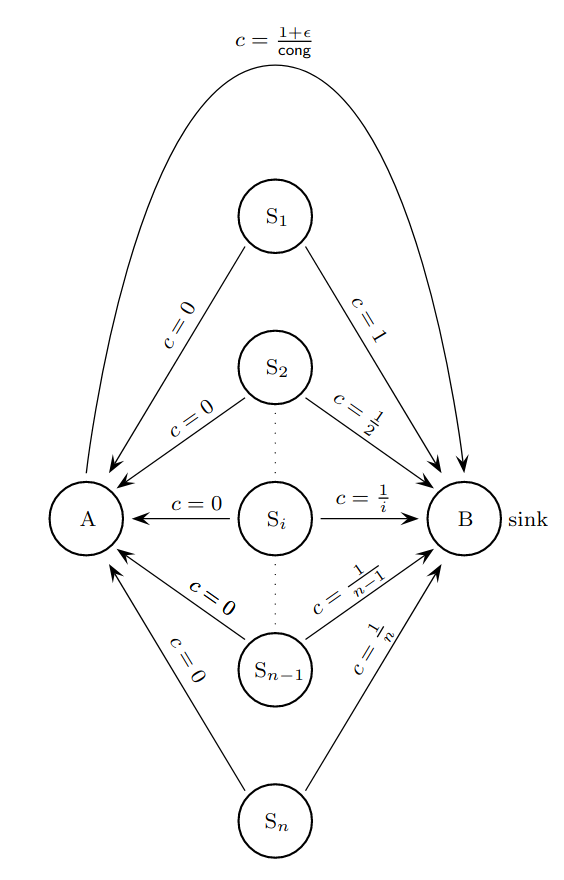
\includegraphics[width=0.7\textwidth]{images/img_3_16_01.png}
\end{figure}
There are $n$ players, each player $i$ starting from node $S_i$. There is only one sink that is node $B$. All the players using an edge (corresponding to a resource) share uniformly the cost. Notice that all the edges can be used by only one player, except the edge connecting node $A$ to node $B$ that, in principle, can be used by all the players.Let $k$ to be the users using such an edge, the cost of each user is $(1 + \epsilon)/k$. The PoS of the above game in unbounded, asymptotically depending logarithmically on $n$. The socially best solution is when all the players move to $A$ and then to $B$, with a social cost of $1+\epsilon$. Each player has a cost of $(1 + \epsilon)/n$. This is not a Nash equilibrium, since player $n$ strictly prefers to go directly to $B$, with a cost of $1/n$. Once player $n$ changed her action, player $n-1$ does the same. Indeed, $(1+\epsilon)/(n-1)$ is strictly larger than $1/(n-1)$. The same happens for all the other players. The only possible Nash equilibrium is when each player moves directly to $B$, with a social cost of $\sum_{i=1}^{n}{\frac{1}{i}}$. Therefore, we have that $\sum_{i=1}^{n}{\frac{1}{i}} = \Theta(\ln (n))$ goes to infinity.\\

\textbf{Exercise 16.0.9} (Upper bound over best-response paths length). \textit{Provide an upper bound over the length of best-response paths in singleton congestion games and prove it.}\\

(Singleton congestion game).A congestion game is called singleton if, for every player $i$ all the actions $a_i \in A_i$ contain a single resource.\\
(Upper bound over the best-response paths). In a singleton congestion game with $n$ players and $m$ resources, best-response paths have length $O(n?2 m)$.\\
\textit{Proof}. We know that any singleton congestion game with $n$ players and $m$ resources is equivalent to a game with $n$ players and $m$ resources in which the maximum cost is $nm$. It can be easily showed that $	Phi$ is upper bounded by $n^2 m$. Indeed, we have:
$$\Phi(\mathbf{a})=\sum_{j=1}^{m} \sum_{k=1}^{\operatorname{cong}_{j}(\mathbf{a})} c_{j}(k)=\sum_{j=1}^{m} \sum_{k=1}^{\operatorname{cong}_{j}(\mathbf{a})} n m=n^{2} m$$
Furthermore, along best-response paths $\Delta \Phi \leqslant 1$ since each pair of costs differs for at least 1. Since $\Phi$ strictly reduces along best-response paths, no best-response path can be longer than $n^2 m$.

\section{EC 3.17}
\textbf{Exercise 17.0.1} (Social choice functions). \textit{Provide the definition of social choice function. Provide one example.}\\

A social choice function $f: \Theta_1 \times \ldots \times \Theta_n \rightarrow X$ assigns an outcome $x$ to each possible profile of players' types.\\

\textbf{Exercise 17.0.2} (Efficiency). \textit{Provide the definitions of ex ante, ex interim, ex post efficiency for social choice functions. Answer to the following questions.
\begin{itemize}
\item Is the social choice function implemented by the Second-Price auction efficient in ex post?
\item Provide an example of social choice function that is efficient in ex post, but not in ex interim.
\item Provide an example of social choice function that is efficient in ex interim, but not in ex post.\\
\end{itemize}}

(Ex post efficiency). A social choice function $f: \Theta_{1} \times \ldots \times \Theta_{n} \rightarrow X$ is ex post efficient if there is no other social choice function $f^{\prime}$ such that:
$$
\begin{array}{ll}
\forall i \in N, \forall \theta \in \Theta: & U_{i}\left(f^{\prime}(\theta), \theta_{i}\right) \geqslant U_{i}\left(f(\theta), \theta_{i}\right) \quad \text { and } \\
\exists i \in N, \exists \theta \in \Theta: & U_{i}\left(f^{\prime}(\theta), \theta_{i}\right)>U_{i}\left(f(\theta), \theta_{i}\right)
\end{array}
$$

(Ex interim efficiency). A social choice function $f: \Theta_{1} \times \ldots \times \Theta_{n} \rightarrow X$ is ex interim efficient if there is no other social choice function $f^{\prime}$ such that:
$$
\begin{array}{ll}
\forall i \in N, \forall \theta_{i} \in \Theta_{i}: & \mathbb{E}_{\theta_{-i}}\left[U_{i}\left(f^{\prime}(\theta), \theta_{i}\right)\right] \geqslant \mathbb{E}_{\theta_{-i}}\left[U_{i}\left(f(\theta), \theta_{i}\right)\right] \text { and } \\
\exists i \in N, \exists \theta_{i} \in \Theta_{i}: & \mathbb{E}_{\theta_{-i}}\left[U_{i}\left(f^{\prime}(\theta), \theta_{i}\right)\right]>\mathbb{E}_{\theta_{-i}}\left[U_{i}\left(f(\theta), \theta_{i}\right)\right]
\end{array}
$$
(Ex ante efficiency). A social choice function $f: \Theta_{1} \times \ldots \times \Theta_{n} \rightarrow X$ is ex ante efficient if $f$ there no other social choice function $f^{\prime}$ such that:
$$
\begin{array}{ll}
\forall i \in N: & \mathbb{E}_{\theta}\left[U_{i}\left(f^{\prime}(\theta), \theta_{i}\right)\right] \geqslant \mathbb{E}_{\theta}\left[U_{i}\left(f(\theta), \theta_{i}\right)\right] \text { and } \\
\exists i \in N: & \mathbb{E}_{\theta}\left[U_{i}\left(f^{\prime}(\theta), \theta_{i}\right)\right]>\mathbb{E}_{\theta}\left[U_{i}\left(f(\theta), \theta_{i}\right)\right]
\end{array}
$$

(Ex post efficiency).Consider the above social choice functions:
\begin{itemize}
\item Continuous voting with average allocation: it is ex post efficient. Indeed, moving away from the outcome chosen by $f$, the utility of at least one player decreases.
\item Continuous voting with median allocation: it is ex post efficient. Indeed, moving away from the outcome chosen by $f$, the utility of at least one player decreases.
\item Auction without payments: it is ex post efficient. Indeed, each outcome is Pareto efficient.
\item First-price auction: it is not ex post efficient. Indeed $f'$ defined in the auction without payments Pareto dominates $f$ defined in first-price auction.
\item Second-price auction: it is not ex post efficient. Indeed $f'$ defined in the auction without payments Pareto dominates $f$ defined in second-price auction.
\end{itemize}

\textbf{Exercise 17.0.3} (Individual rationality). \textit{Provide the definitions of ex ante, ex interim, ex post individual rationality for social choice functions. Answer to the following questions.
\begin{itemize}
\item Is the social choice function implemented by the Second-Price auction individually rational in ex post?
\item Provide an example of social choice function that is individually rational in ex interim, but not in ex post.
\item Provide an example of social choice function that is individually rational in ex ante, but not in ex interim.
\item Provide an example of social choice function that is individually rational in ex interim, but not in ex ante.\\
\end{itemize}}

(Ex post individually rationality). A social choice function $f: \Theta_{1} \times \ldots \times \Theta_{n} \rightarrow X$ is ex post individually rational if:
$$
\forall i \in N, \forall \theta \in \Theta: \quad U_{i}\left(f(\theta), \theta_{i}\right) \geqslant \bar{U}_{i}\left(\theta_{i}\right)
$$
where $\bar{U}_{i}\left(\theta_{i}\right)$ is the utility of player $i$ when her type is $\theta_{i}$ and she does not participate to the social choice.

(Ex interim individually rationality). A social choice function $f: \Theta_{1} \times \ldots \times \Theta_{n} \rightarrow X$ is ex interim individually rational if:
$$
\forall i \in N, \forall \theta_{i} \in \Theta_{i}: \quad \mathbb{E}_{\theta_{-i}}\left[U_{i}\left(f(\theta), \theta_{i}\right)\right] \geqslant \bar{U}_{i}\left(\theta_{i}\right)
$$
where $\bar{U}_{i}\left(\theta_{i}\right)$ is the utility of player $i$ when her type is $\theta_{i}$ and she does not participate to the social choice.

(Ex ante individually rationality). A social choice function $f: \Theta_{1} \times \ldots \times \Theta_{n} \rightarrow X$ is ex ante individually rational if:
$$
\forall i \in N: \quad \mathbb{E}_{\theta}\left[U_{i}\left(f(\theta), \theta_{i}\right)\right] \geqslant \mathbb{E}_{\theta}\left[\bar{U}_{i}\left(\theta_{i}\right)\right]
$$
where $\bar{U}_{i}\left(\theta_{i}\right)$ is the utility of player $i$ when her type is $\theta_{i}$ and she does not participate to the social choice.
 
(Ex post individually rationality). Consider the above social choice functions, under the assumption that $bar{U}_{i}\left(\theta_{i}\right)=0$ for every $i \in N$ and $\theta_i \in \Theta_i$:
\begin{itemize}
\item Continuous voting with average allocation: it is ex post individually rational. Indeed, for every outcome $x \in X$ the utility of each player is not negative.
\item Continuous voting with median allocation: it is ex post individually rational. Indeed, for every outcome $x \in X$ the utility of each player is not negative.
\item Auction without payments: it is ex post individually rational. Indeed, each outcome provides each player with a non-negative utility.
\item First-price auction: it is ex post individually rational. Indeed, each outcome provides each player with a non-negative utility.
\item Second-price auction: it is ex post individually rational. Indeed, each outcome provides each player with a non-negative utility.
\end{itemize}

\textbf{Exercise 17.0.4} (Dictatorship). \textit{Provide the definition of dictatorship for social choice functions. Provide an example.}\\

A social choice function $f: \Theta_{1} \times \ldots \times \Theta_{n} \rightarrow X$ is dictatorial if there is a player $i$ (said dictator) such that for every $\theta \in \Theta$ it holds:
$$
U_{i}\left(f(\theta), \theta_{i}\right) \geqslant U_{i}\left(x, \theta_{i}\right) \quad \forall x \in X
$$

\section{EC 3.18}

\textbf{Exercise 18.0.1} (Economic mechanism). \textit{Provide the definition of economic mechanism.}\\

An economic mechanism is a tuple $(A_1,\ldots,A_n,X,g)$ where:
\begin{itemize}
\item $A_i$ is the set of actions of player $i$;
\item $X$ is the set of outcomes;
\item $g: A_1 \times \ldots \times A_n\rightarrow X$ is the outcome function.
\end{itemize} 

\textbf{Exercise 18.0.2} (Implementation of a social choice function). \textit{Provide the definition of implementation of a social choice function.}\\

An economic mechanism $\left(A_{1}, \ldots, A_{n}, X, g\right)$ implements a social choice function $f: \Theta_{1} \times \ldots \times \Theta_{n} \rightarrow X$ if there is a pure-strategy equilibrium (according to
some solution concept) strategy profile $\left(s_{1}^{*}, \ldots, s_{n}^{*}\right)$ of the Bayesian game induced by the economic mechanism such that:
$$
g\left(s_{1}^{*}\left(\theta_{1}\right), \ldots, s_{n}^{*}\left(\theta_{n}\right)\right)=f\left(\theta_{1}, \ldots, \theta_{n}\right) \text { for every }\left(\theta_{1}, \ldots, \theta_{n}\right) \in \Theta_{1} \times \ldots \times \Theta_{n}
$$
where $s_{i}^{*}\left(\theta_{i}\right)$ denotes the optimal strategy of player i when her type is $\theta_{i}$.\\

\textbf{Exercise 18.0.3} (Direct-revelation mechanism). \textit{Provide the definitions of direct-revelation mechanism and indirect-revelation mechanism and provide an example for each one of them.}\\

(Direct (revelation) economic mechanism). Given a social choice function $f: \Theta_{1} \times \ldots \times \Theta_{n} \rightarrow$ $X$, a direct (revelation) economic mechanism is a mechanism $\left(\Theta_{1}, \ldots, \Theta_{n}, X, f\right)$

(Direct (revelation) economic mechanism). $A$ direct mechanism is an economic mechanism in which the actions available to each player $i$ are given by the set of types of player $i$ (i.e., each player can only report a type from the set of the possible ones) and the outcome function is a social choice function.

(Indirect (revelation) economic mechanism). An economic mechanism that is not direct is said indirect.\\

\textbf{Exercise 18.0.4} (Incentive compatibility). \textit{Provide the definition of incentive compatibility.}\\

A social choice function $f: \Theta_{1} \times \ldots \times \Theta_{n} \rightarrow$ $X,$ is incentive compatible (or truthfully implementable) if the Bayesian game induced by the direct revelation economic mechanism $(\Theta_{1}, \ldots, \Theta_{n}, X, f)$ has a pure equilibrium (according to some solution concept) $(s^*_1, \ldots, s^*_n)$ such that $s^*_i (\theta_i) = \theta_i$ for every player $i$ and type $\theta_i$. (And therefore the direct revelation economic mechanism $(\Theta_{1}, \ldots, \Theta_{n}, X, f)$ implements $f$).

Incentive compatibility can be satisfied according to different solution concepts, among them:
\begin{itemize} 
\item Dominant-strategy incentive compatibility (DSIC): if $(s^*_1, \ldots, s^*_n)$ where $s^*_i (\theta_i) = \theta_i$ for every player $i$ and type profile $\theta_i$ is a (weak) Dominant-Strategy equilibrium;
\item Bayesian incentive compatibility (BNIC): if $(s^*_1, \ldots, s^*_n)$ where $s^*_i (\theta_i) = \theta_i$ for every player $i$ and type $\theta_i$ is a Bayes-Nash equilibrium.
\end{itemize}

\textbf{Exercise 18.0.5} (Checking incentive compatibility). \textit{Given a social choice function, check whether it is incentive compatible.}\\

\textcolor{red}{TODO}\\

\textbf{Exercise 18.0.6} (Revelation principle for Dominant-Strategy equilibrium). \textit{Provide the statement of the revelation principle and the proof.}\\

Given a social choice function $f: \Theta_{1} \times \ldots \times \Theta_{n} \rightarrow X$, if there is an economic mechanism $\left(A_{1}, \ldots, A_{n}, X, g\right)$ implementing $f$ in Dominant Strategy equilibrium, then $f$ is DSIC.
Proof. If $\left(A_{1}, \ldots, A_{n}, X, g\right)$ implements $f$ in Dominant-Strategy equilibrium, then there is a strategy profile $\left(s_{1}^{*}, \ldots, s_{n}^{*}\right)$ such that:
$$
g\left(s_{1}^{*}\left(\theta_{1}\right), \ldots, s_{n}^{*}\left(\theta_{n}\right)\right)=f\left(\theta_{1}, \ldots, \theta_{n}\right) \quad \forall\left(\theta_{1}, \ldots, \theta_{n}\right) \in \Theta
$$
and
$$
U_{i}\left(g\left(s_{i}^{*}\left(\theta_{i}\right), s_{-i}\left(\theta_{-i}\right)\right), \theta_{i}\right) \geqslant U_{i}\left(g\left(s_{i}\left(\theta_{i}\right), s_{-i}\left(\theta_{-i}\right)\right), \theta_{i}\right) \quad \forall i \in N, \theta_{i} \in \Theta_{i}, \theta_{-i} \in \Theta_{-i}, s_{i}, s_{-i}
$$
The above condition is obviously satisfied for any restriction over $s_{i}$ and $s_{-i} .$ Thus, we fix $s_{i}\left(\theta_{i}\right)=s_{i}^{*}\left(\hat{\theta}_{i}\right)$ (that is, we are restricting $s_{i}\left(\theta_{i}\right)$ to the set of the optimal strategies $s_{i}^{*}$ allowing player $i$ to select the strategy just by misreporting the type) and we fix $s_{-i}\left(\theta_{-i}\right)=s_{-i}^{*}\left(\theta_{-i}\right)$ (that is, we are restricting $s_{-i}\left(\theta_{-i}\right)$ to the set of the optimal strategies $\left.s_{-i}^{*}\left(\theta_{-i}\right)\right)$. We obtain:
$$
U_{i}\left(g\left(s_{i}^{*}\left(\theta_{i}\right), s_{-i}^{*}\left(\theta_{-i}\right)\right), \theta_{i}\right) \geqslant U_{i}\left(g\left(s_{i}^{*}\left(\hat{\theta}_{i}\right), s_{-i}^{*}\left(\theta_{-i}\right)\right), \theta_{i}\right) \quad \forall i \in N, \theta_{i} \in \Theta_{i}, \theta_{-i} \in \Theta_{-i}, \hat{\theta}_{i} \in \Theta_{i}
$$
Now we substitute $g\left(s_{i}^{*}\left(\theta_{i}\right), s_{-i}^{*}\left(\theta_{-i}\right)\right)$ with $f\left(\theta_{i}, \theta_{-i}\right)$ and $g\left(s_{i}^{*}\left(\hat{\theta}_{i}\right), s_{-i}^{*}\left(\theta_{-i}\right)\right)$ with $f\left(\hat{\theta}_{i}, \theta_{-i}\right)$, obtaining:
$$
U_{i}\left(f\left(\theta_{i}, \theta_{-i}\right), \theta_{i}\right) \geqslant U_{i}\left(f\left(\hat{\theta}_{i}, \theta_{-i}\right), \theta_{i}\right) \quad \forall i \in N, \theta_{i} \in \Theta_{i}, \theta_{-i} \in \Theta_{-i}, \hat{\theta}_{i} \in \Theta_{i}
$$
This condition exactly corresponds to the condition of incentive compatibility in dominant strategies.\\

\textbf{Exercise 18.0.7} (Gibbard-Satterthwaite impossibility theorem). \textit{Provide the statement of the Gibbard-Satterthwaite impossibility theorem.}\\

Given a social choice function $f: \Theta_{1} \times \ldots \times \Theta_{n} \rightarrow X$, if
\begin{itemize}
\item $X$ is finite and $|X| \leqslant 3$,
\item $f$ is onto (surjective),
\item the utility functions of all the players cover the entire space of strict-preference utility functions, then the social choice function $f$ is DSIC if and only if it is dictatorial.
\end{itemize}
